Negli algoritmi visti fin'ora, per trovare la policy adatta ($a = \pi(s)$ dove con $\pi$ indichiamo appunto la \textit{policy}) siamo sempre andati ad utilizzare una funzione approssimata $Q_{\pi^*}(s,a)$, la quale permetteva all'agente di scegliere quale fosse l'azione migliore da compiere, sia nel caso di azioni discrete, sia nel caso di azioni continue che discrete ()come si vede in figura ~\ref{fig:Q_function_utility}) andando poi a selezionare l'azione in grado di massimizzare l'output.

\begin{figure}[!h]
	\centering
	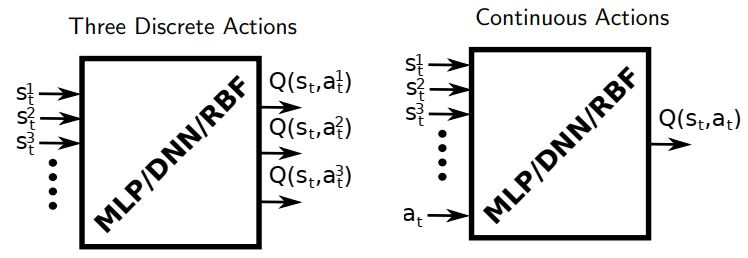
\includegraphics[width=0.8\textwidth]{Immagini/Q_function_utility.JPG}
	\caption{Valutazione della funzione sulla base della Q-values}
	\label{fig:Q_function_utility}
\end{figure}

La domanda che ci poniamo è: \textit{possiamo trovare la policy direttamente} partendo dallo stato attuale ($s_t$) e ottenendo appunto $a_t$?

La risposta è si.

\begin{figure}[!h]
	\centering
	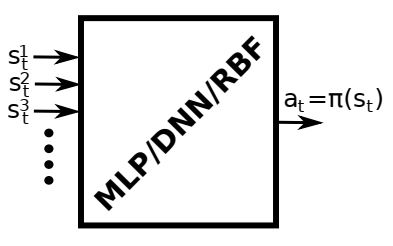
\includegraphics[width=0.5\textwidth]{Immagini/No_Q_function.JPG}
	\caption{Valutazione della funzione \textit{non} basandosi sulla Q-values}
	\label{fig:NO_Q_function_utility}
\end{figure}
Questo concetto, mostrato in maniera molto diretta nella figura ~\ref{fig:NO_Q_function_utility}, è quello che nella letteratura del RL viene chiamato come metodo di \textit{policy search}, il quale permette appunto di stimare la polici ottimale ($\pi^*(a|s)$) invece di cercare il valore ottimo per la funzione $Q^*(s,a))$: questo nuovo approccio presenta innumerevoli vantaggi rispetto agli algoritmi mostrati in precedenza, in particolare:
\begin{itemize}
	\item Policies ottimali, scelte tramite algoritmi di questo tipo, presentano un numero di parametri minore rispetto al valore ottimale della q-functions (\textit{curse of dimensionality})
	\item Processo di learn più veloce (e questo è anche dimostrato dai grafici presenti all'interno di questa documentazione)
	\item Offre la possibilità di utilizzare policies sia deterministiche che stocastiche (\textit{noisly})
\end{itemize}

\textit{E cosa cerchiamo di ottimizzare in questo nuovo contesto?}
I metodi di policy search vanno ad ottimizzare l'indice $J(\theta)$, dove $\theta$ rappresenta il vettore dei pesi; è possibile realizzare questa ottimizzazione utilizzando differenti metodi:
\begin{itemize}
	\item Gradient free methods:
	\begin{itemize}
		\item Evolutionary computation
		\item Simulated annealing
		\item Hill climbing
	\end{itemize}
	\item \textbf{Gradient based methods} (\textit{policy gradient methods}):
	\begin{itemize}
		\item  Gradient estimation 
		\item Optimization algorithm
	\end{itemize}
\end{itemize}

I passi principali che sono stati implementati, sono
\begin{itemize}
	\item Implementare la dinamica del carrello (di cui non si riporta la trattazione) e una funzione per simulare i roll-outs (sotto sezione ~\ref{sec:rollout}) che forniscono il reward di ritorno;
	\item Utilizzare una \textit{Radial Basis Function} (RBF network - sotto sezione ~\ref{sec:RBF}) per approssimare l'apprendimento, ovvero per ottenere $a = \pi(s,W) = W^T\Phi(s,a)$
	\item Implementare l'algoritmo alla differenze finite (FD) per apprendere i pesi della policy
\end{itemize}

\subsection{Approccio \textit{Policy gradient estimation}}
Come già sottolineato in precedenza andremo a basarci su un algoritmo \textit{gradient based}, nello specifico l'agoritmo alla differenze finite, il quale, in ambito matematico, rappresenta una strategia utilizzata per risolvere numericamente equazioni differenziali che si basa sull'approssimazione delle derivate con equazioni alle differenze finite.

Questa approssimazione che andiamo ad utilizzare per effettuare un'operazione di minimizzazione (anche locale) sulla funzione $J(\theta) = V_\pi(s)$ \label{eq:J_function_to_minimize}: l'approccio che si è deciso di seguire non è però quello classico, ma bensì una strada alternativa, in cui, fornita una policy parametrizzata $\pi(a|s,\theta)$, possiamo calcolare $J(\theta)$ simulando l'environment come un \textit{Markov Decision Process}, la funzione $J(\theta)$. 

In particolare:
\begin{itemize}
	\item Invece di calcolare $\partial V / \partial\phi_i$ separatamente (passaggio che verrebbe naturale dopo aver definito $J(\theta)$ in \ref{eq:J_function_to_minimize}), andiamo ad ottenere un vettore random $\delta ~ N (0, \sigma^2)$.
	Nel codice questa parte è stata implementata in questo modo:
	\begin{lstlisting}
	# Variance of the random Gaussian perturbation of the parameters
	variance_of_perturbation = 0.1 
	# random parameter 	variation (Gaussian)
	delta = variance_of_perturbation * np.random.randn(numberOfCentrum, 1) 
	\end{lstlisting}
	\item Il vettore randomico generato in precedenza lo utilizzeremo poi per calcolare, tramite la tecnica definita \textit{roll-out} (sezione ~\ref{sec:rollout}), due valori della funzione J ($J_+, J_-$)
	\item Utilizzando l'approssimazione di taylor possiamo scrivere $J_+ \approx J(\Theta) + \nabla J^T \delta$ e $J_- \approx J(\Theta) - \nabla J^T \delta$
	\item La differenza $J_\Delta = J_+ - J_-$ diventa $J_\Delta = 2 \delta^T \nabla J$, dove $J_\Delta$ è un numero scalare mentre $\nabla J$ e $\delta$ sono vettori.
\end{itemize}

Questo processo andiamo a ripeterlo più volte con differenti valori randomici di $\delta_i$ con $i= 1,2,...N_H$: andremo quindi ad ottenere così differenti $J_{\Delta_i}$, ma ci sarà solamente un gradiente ($\nabla J$ sconosciuto).

In forma matriciale quindi diventa:
\begin{figure}[h!]
	\centering
	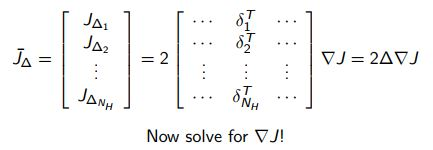
\includegraphics[width=0.7\textwidth]{Immagini/Matrix_form.JPG}
	\caption{Matrix form}
	\label{fig:matrix_form}
\end{figure}
La soluzione dovrebbe essere data da $\nabla J = 1/2 \Delta^{-1} J_\Delta$, ma $\Delta$
potrebbe non essere una matrice quadrata (per il fatto che il numero di rollout potrebbe non essere pari alla dimensione di $\Theta$): con alcuni passaggi matematici (qui omessi) possiamo andare una forma più stabile per ricavare la soluzione (riportata anche in precedenza) data da $\Delta J = 1/2 [\Delta^T \Delta +\lambda I]^{-1} \Delta^T J_\Delta$
\newpage
\subsection{Algoritmo \textit{FD}}
Questo è l'algoritmo implementato nel codice per apprendere i parametri ottimi. 
La corrispondeza implementata in \textit{Python} dell'algoritmo ~\ref{alg:FD_alg} la si trova nella figura ~\ref{fig:FD_py_alg}.

\begin{algorithm} [h!]
	\SetAlgoLined
	\caption{Finite Differences algorithm}
	\label{alg:FD_alg}
	\KwIn{Input: approssimazione della funzione parametrica $\pi(\bullet,\bullet,\Theta)$}
	\KwOut{Output: pesi ottimali $\Theta^*$}
	\KwData{Parametri: \textit{Learning rate $\alpha$}, $\lambda$, $\sigma_\delta ^2$, numero di rollout}
	\While{Policy non converge}{
		Inizializza $J_\Delta$ e $\Delta$
		
		\For{$i = 1,2,..., N_H$}{
			Inizializza lo stato iniziale $s_0$
			
			Genera una variazione randomica $\delta$ distribuita come $N(0,\sigma_\delta^2)$
			
			$J_+ \leftarrow rollout(\pi(\Theta + \delta))$
			
			$J_- \leftarrow rollout(\pi(\Theta - \delta))$
			
			Add $J_+ - J_-$ al parametro  $J_\Delta$
			
			Add $\delta^T$ a $\Delta$
		}
		$\Theta^* \leftarrow \Theta^* + 1/2\alpha [\Delta^T \Delta + \lambda I]^{-1} \Delta^T J_\Delta$
	}
\end{algorithm}

\begin{figure}[!h]
	\centering
	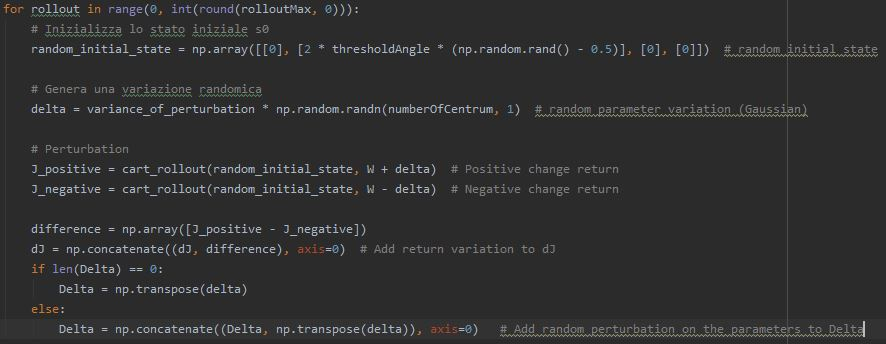
\includegraphics[width=\textwidth]{Immagini/FD_alg_python.JPG}
	\caption{Reward \textit{Finite Differences in Python}}
	\label{fig:FD_py_alg}
\end{figure}

\subsubsection{Rollout}
\label{sec:rollout}
Fornita una policy $a = \pi(s)$ oppure $a = \pi(a|s)$ e uno stato iniziale $s_0$ ad un certo istante temporale di un \textit{Markov Decision Process}, un rollout (definibile anche come \textit{traiettoria, storia o trial}), è semplicemente una sequenza \textbf{$H = s_0, a_0, s_1, a_1, .. , s_T, a_T$} generata a partire da uno stato $s_0$ e seguendo una policy $\pi$.
Nella implementazione relativa a questo progetto, come spiegato nella sotto sezione ~\ref{sec:RBF}, siamo andati ad utilizzare come approssimazione della policy da seguire il risultato fornito in uscita da una \textit{Radial Basis Function} neural network. 

\begin{figure}[!h]
	\centering
	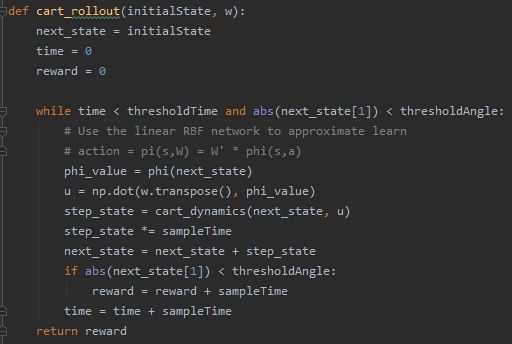
\includegraphics[width=0.7\textwidth]{Immagini/Rollout.JPG}
	\caption{Rollout in Python}
	\label{fig:roll_py}
\end{figure}

I pesi di questa rete neurale, come si può vedere nell'implementazione in figura ~\ref{fig:roll_py}, risultano però essere fissati, il che quindi equivale all'andare a seguire sempre la stessa policy.
\subsubsection{RBF network}
\label{sec:RBF}
Come è stato evidenziato in precedenza, siamo andati ad utilizzare una \textit{RBF} lineare per andare ad approssimare l'apprendimento.

In particolar modo le \textit{Radial Basis Function} permettono di andare a partizionare lo spazio degli stati, sovrapponendo dei \textit{"Gaussian neurons"}, in cui ogni neurone genera un segnale corrispondente al vettore di input: il segnale prodotto da ogni neurone presenta una potenza che dipende dalla distanza tra il centro della curva gaussiana che rappresenta il vettore e il vettore degli stati in input.

Questo concetto base delle \textit{RBF} viene implementato andando a creare una tabella formata da una sequenza di punti cartesiani, i quali rappresentano i centri di ognuno dei neuroni della rete neurale, ovvero la media di ogni curva gaussiana (figura ~\ref{fig:RBF_Centrum}).

\begin{figure}[!h]
	\centering
	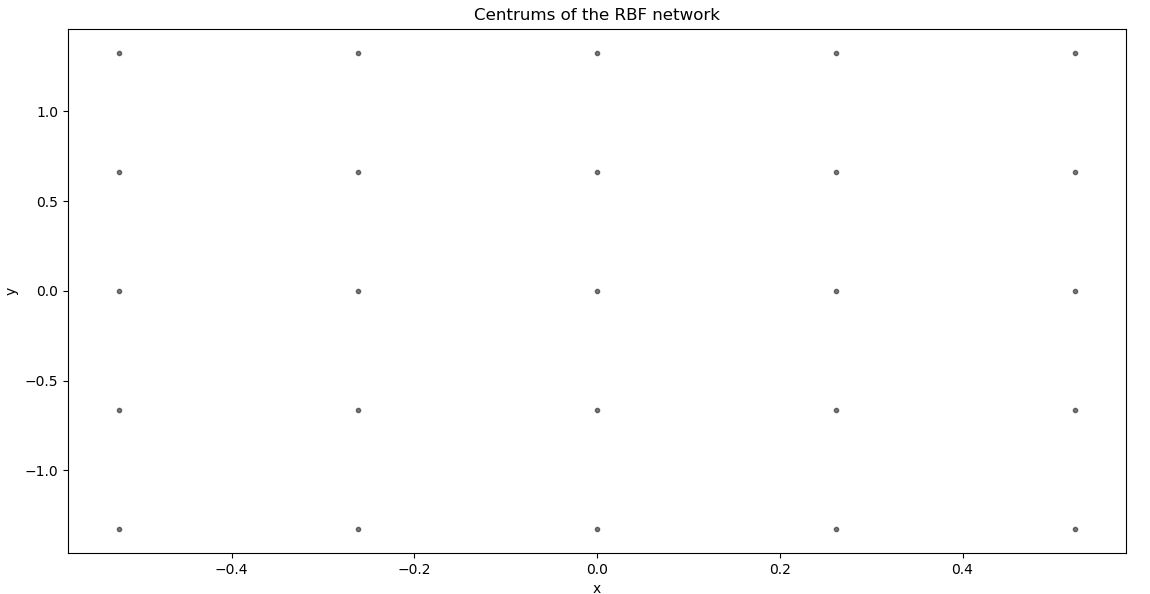
\includegraphics[width=0.5\textwidth]{Immagini/Centrum_of_RBF.JPG}
	\caption{Centri di ogni neurone della \textit{RBF}}
	\label{fig:RBF_Centrum}
\end{figure}

Un altro aspetto importante da evidenziare è il fatto che, i \textit{weigths} relativi alla \textit{RBF} vengono aggiornati tramite algoritmo Finite Difference: quindi, i

\subsection{Result}
Nella figura ~\ref{fig:Reward_FD}, è rappresentato l'andamento del reward con un batch di 10 trial con 70 iterazioni ciascuno: ogni iterazione può essere eseguita per un massimo di 10 s, nel caso in cui l'esecuzione non fallisce prima (ovvero il pole cade fuori dal range angolare imposto).
Si nota quindi come siano necessarie meno iterazioni, rispetto agli algoritmi precedenti, per ottenere un reward molto buono.

\begin{figure}[!h]
	\centering
	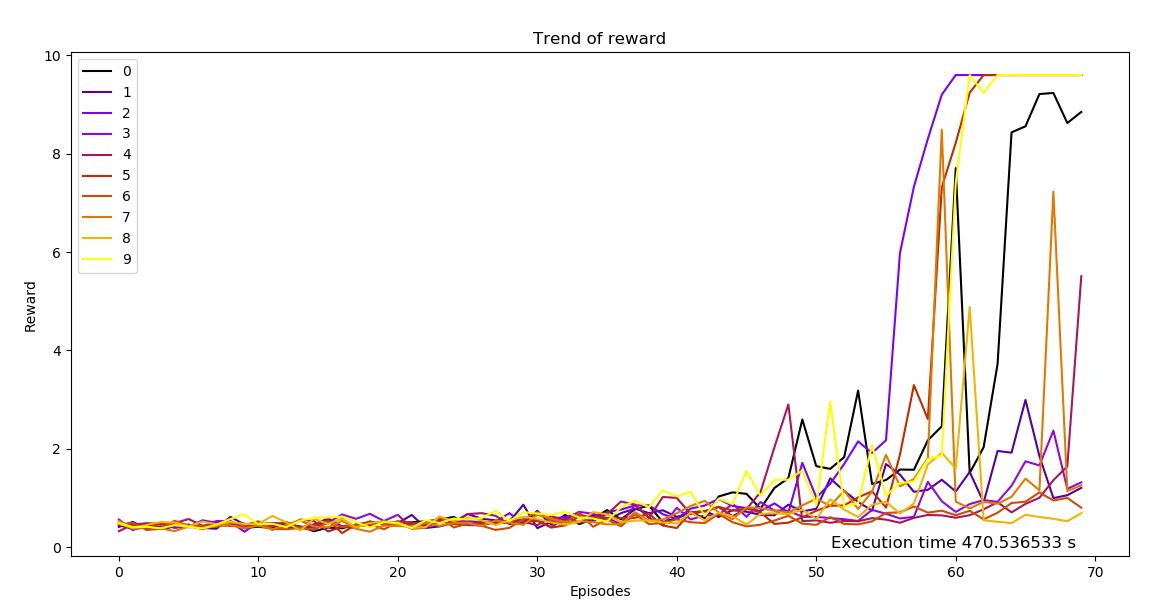
\includegraphics[width=\textwidth]{Immagini/Reward_FD.JPG}
	\caption{Reward \textit{Finite Differences}}
	\label{fig:Reward_FD}
\end{figure}

\newpage